\documentclass[
a4paper,
10pt,
twoside,
% prd,
% aps,
% nofootinbib,
% superscriptaddress,
% floatfix,
% preprintnumbers,
]{article}

% MUST BE RUN WITH LUALATEXMK

\usepackage{preamble}
\usepackage{titleinfo}

\geometry{ % Set document margins
	top			= 2cm,
	bottom		= 2cm,
	left		= 1cm,
	right		= 1cm
}

\newcommand{\mcols}{2} % Choose number of columns (>= 1)


\bibSetup{refs.bib} % Give references file 
% ===== Format headers & footers =====

\pagestyle{fancy}
\fancyhf{}
\fancyhead[LE,RO]{B. Henke}
\fancyhead[LO]{\headertitle\hspace{0.5cm}\textit{PHY981}}
\fancyhead[RE]{\textit{PHY981}\hspace{0.5cm}\headertitle}
\fancyfoot[RE,LO]{\thepage}

\begin{document}
% \tableofcontents
\titleinf{Lipkin Model}
\maketitle
\startmcols


\section{Introduction}\label{sec: intro}


Consider a two level system with the lower energy state ($\sigma = -1$) having an energy of $-\epsilon/2$ and the upper energy state ($\sigma=1$) having an energy of $\epsilon/2$.
Now, consider a another system with $\Omega \in \Z^+$ copies of this two level system.

This gives a system with two quantum numbers, $\sigma \in \{-1,1\}$, and $m \in \{1,2,\dots,\Omega\}$.
In Fock space, the Hamiltonian for this system is
\begin{align}
	\hat{H} &= \frac{1}{2} \epsilon \sum_{m\sigma}\sigma a_{m\sigma}^\dagger a_{m\sigma}- \frac{1}{2}V\sum_{mm'\sigma}a_{m\sigma}^\dagger a_{m'\sigma}^\dagger a_{m'-\sigma}a_{m-\sigma}.
	\label{eq: lipkin_ham_a}
\end{align}
The $V$ term here is the two particle interaction term between adjacent particles.

\section{Quasi-spin Operators} \label{sec: qs operators}

One can consider the operators
\begin{align}
	\hat{K}_3 &= \frac{1}{2} \sum_{m=1}^\Omega (a_{m+}^\dagger a_{m+}-a_{m-}^\dagger a_{m-}),\\
	\hat{K}_+ &= \sum_{m=1}^\Omega a_{m+}^\dagger a_{m-},\\
	\hat{K}_- &= (\hat{K}_+)^\dagger,\\
		&= \sum_{m=1}^\Omega a_{m-}^\dagger a_{m+}.
\end{align}

Using these "quasi-spin" operators, one can write \ref{eq: lipkin_ham_a} as
\begin{align}
	\hat{H} &= \epsilon \hat{K}_3 - \frac{1}{2}V (\hat{K}_+^2+\hat{K}_-^2).
	\label{eq: lipkin_ham_k}
\end{align}

Furthermore, there are two additional "quasi-spin" operators given by the equations:
\begin{align}
	\hat{K}_1 &= \frac{1}{2}(\hat{K}_+ + \hat{K}_-),\\
	\hat{K}_2 &= \frac{1}{2i}(\hat{K}_+ - \hat{K}_-).
\end{align}
These create a "quasi-spin" space, similar to the angular momentum space with three components representing the three spatial dimensions.
One can show that these operators are $SU(2)$ generators, just like the angular momentum operators, by showing that the following commutation relations hold (see the appendix for the algebra):
\begin{align}
	[\hat{K}_+,\hat{K}_-] &= 2\hat{K}_3,\\
	[\hat{K}_3,\hat{K}_\pm] &= \pm\hat{K}_\pm.
\end{align}

\subsection{Signature Operator}\label{ssec: qs-sig}


Consider the quasi-spin vector, $\bm{K}$, where
\begin{align}
	\bm{K}\cdot k_i &= \hat{K}_i,
\end{align}
where $k_i$ are basis vectors in the quasi-spin space.
One can consider a rotation in this space by $\pi$ in some plane of this space.
Let the signature operator be given by
\begin{align}
	\hat{R} &= e^{i\pi\hat{K}_3}.
\end{align}
This operator has the effect of rotating by $\pi$ in the $k_{12}$ plane.

The signature operator commutes with the Hamiltonian ($[\hat{R},\hat{H}] = 0$), so an energy eigenstate is also an eigenstate of the signature operator, with eigenvalue $r \in \{-1,1,-i,i\}$.
If there are an even number of particles, $r\in\{-1,1\}$.
if there are an odd number of particles, $r\in\{-i,i\}$.


\section{Example}\label{sec: example}

Consider a system with 12 particles ($N=12$), $\epsilon = 1$, $\Omega = 12$.
If one imagines "turning on" the interaction term by increasing $V$ from zero, then the energy eigenvalues of the Hamiltonian will begin to diverge, as shown in figure \ref{fig: eigenvalues K6}.
The look of this graph is somewhat reminiscent of the symmetry breaking phase transition for shapes of nuclei.

\begin{figure}[H]
	\centering
	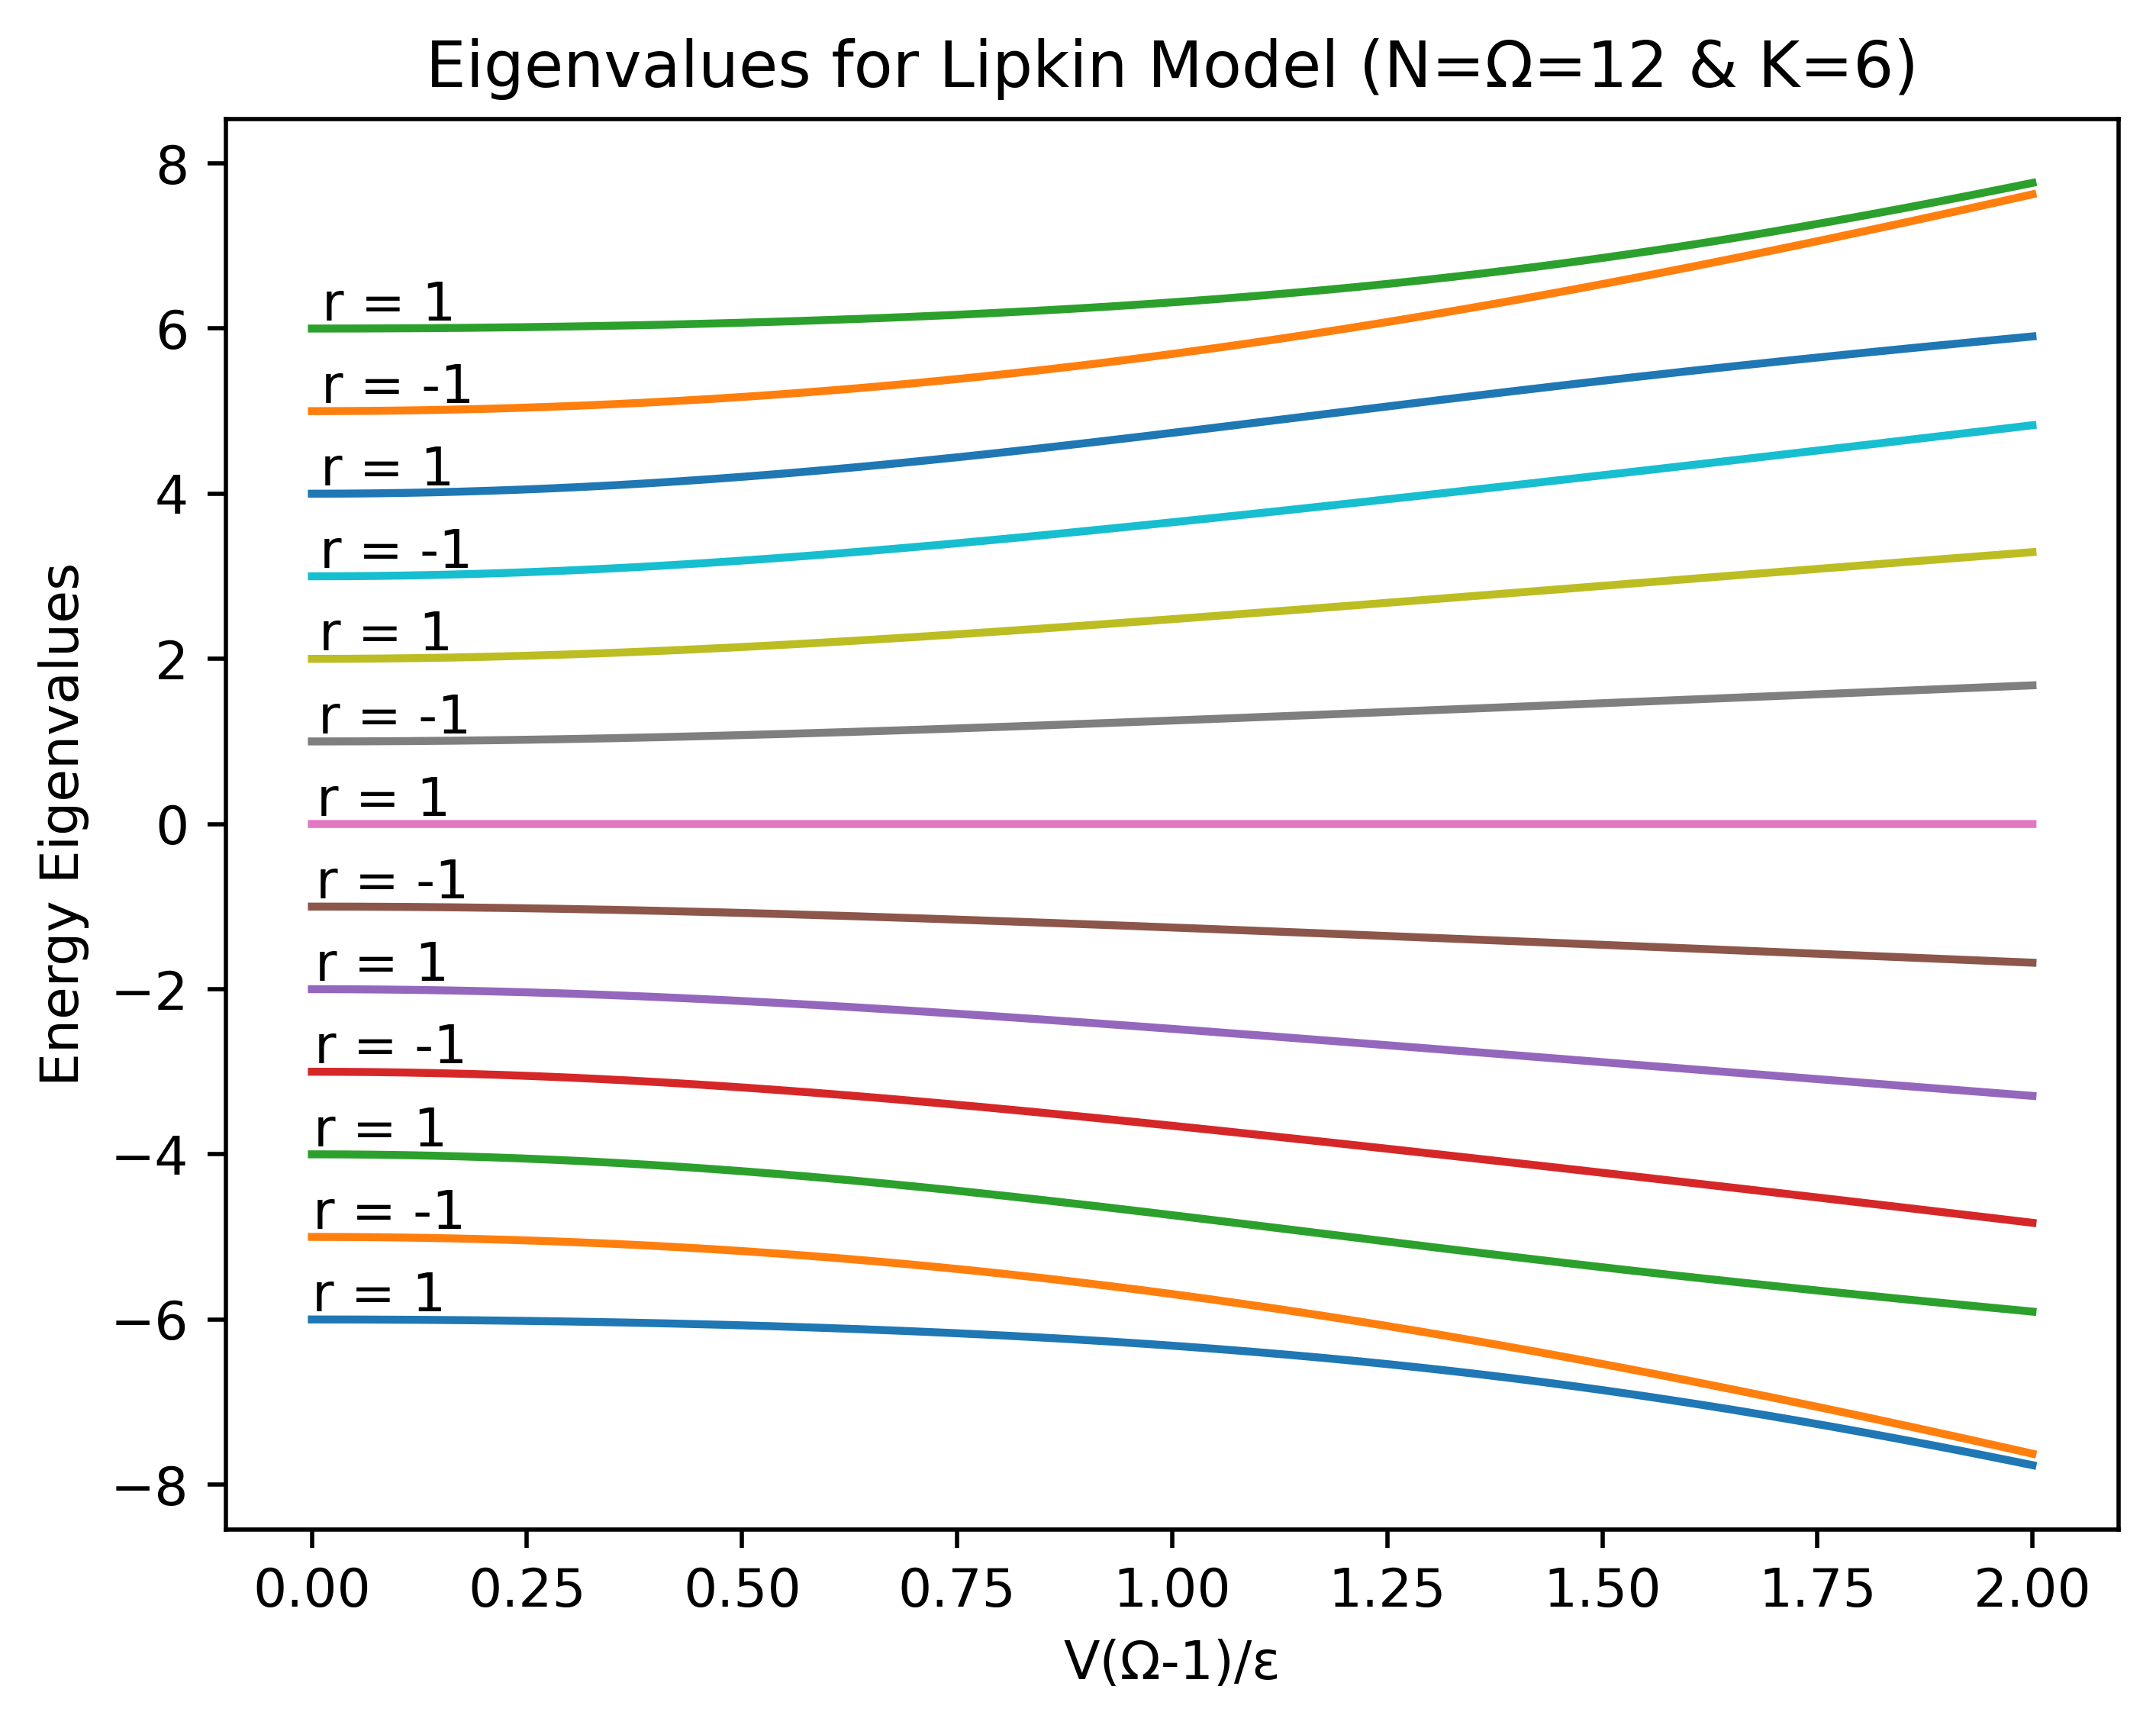
\includegraphics[width=0.8\linewidth]{figures/eigenvaluePlotK6.png}
	\caption{
		Each line in this figure corresponds to an eigenvalue of the Hamiltonian, as the interaction term is "switched on".
		Each line is labeled with the signature eigenvalue, $r$.
		As the interaction term is increased, the eigenvalues begin to diverge.
		The eigenvalues start ($V=0$) evenly spaced by a value of one, but separate as $V$ increases.
	}
	\label{fig: eigenvalues K6}
\end{figure}
\begin{figure}[H]
	\centering
	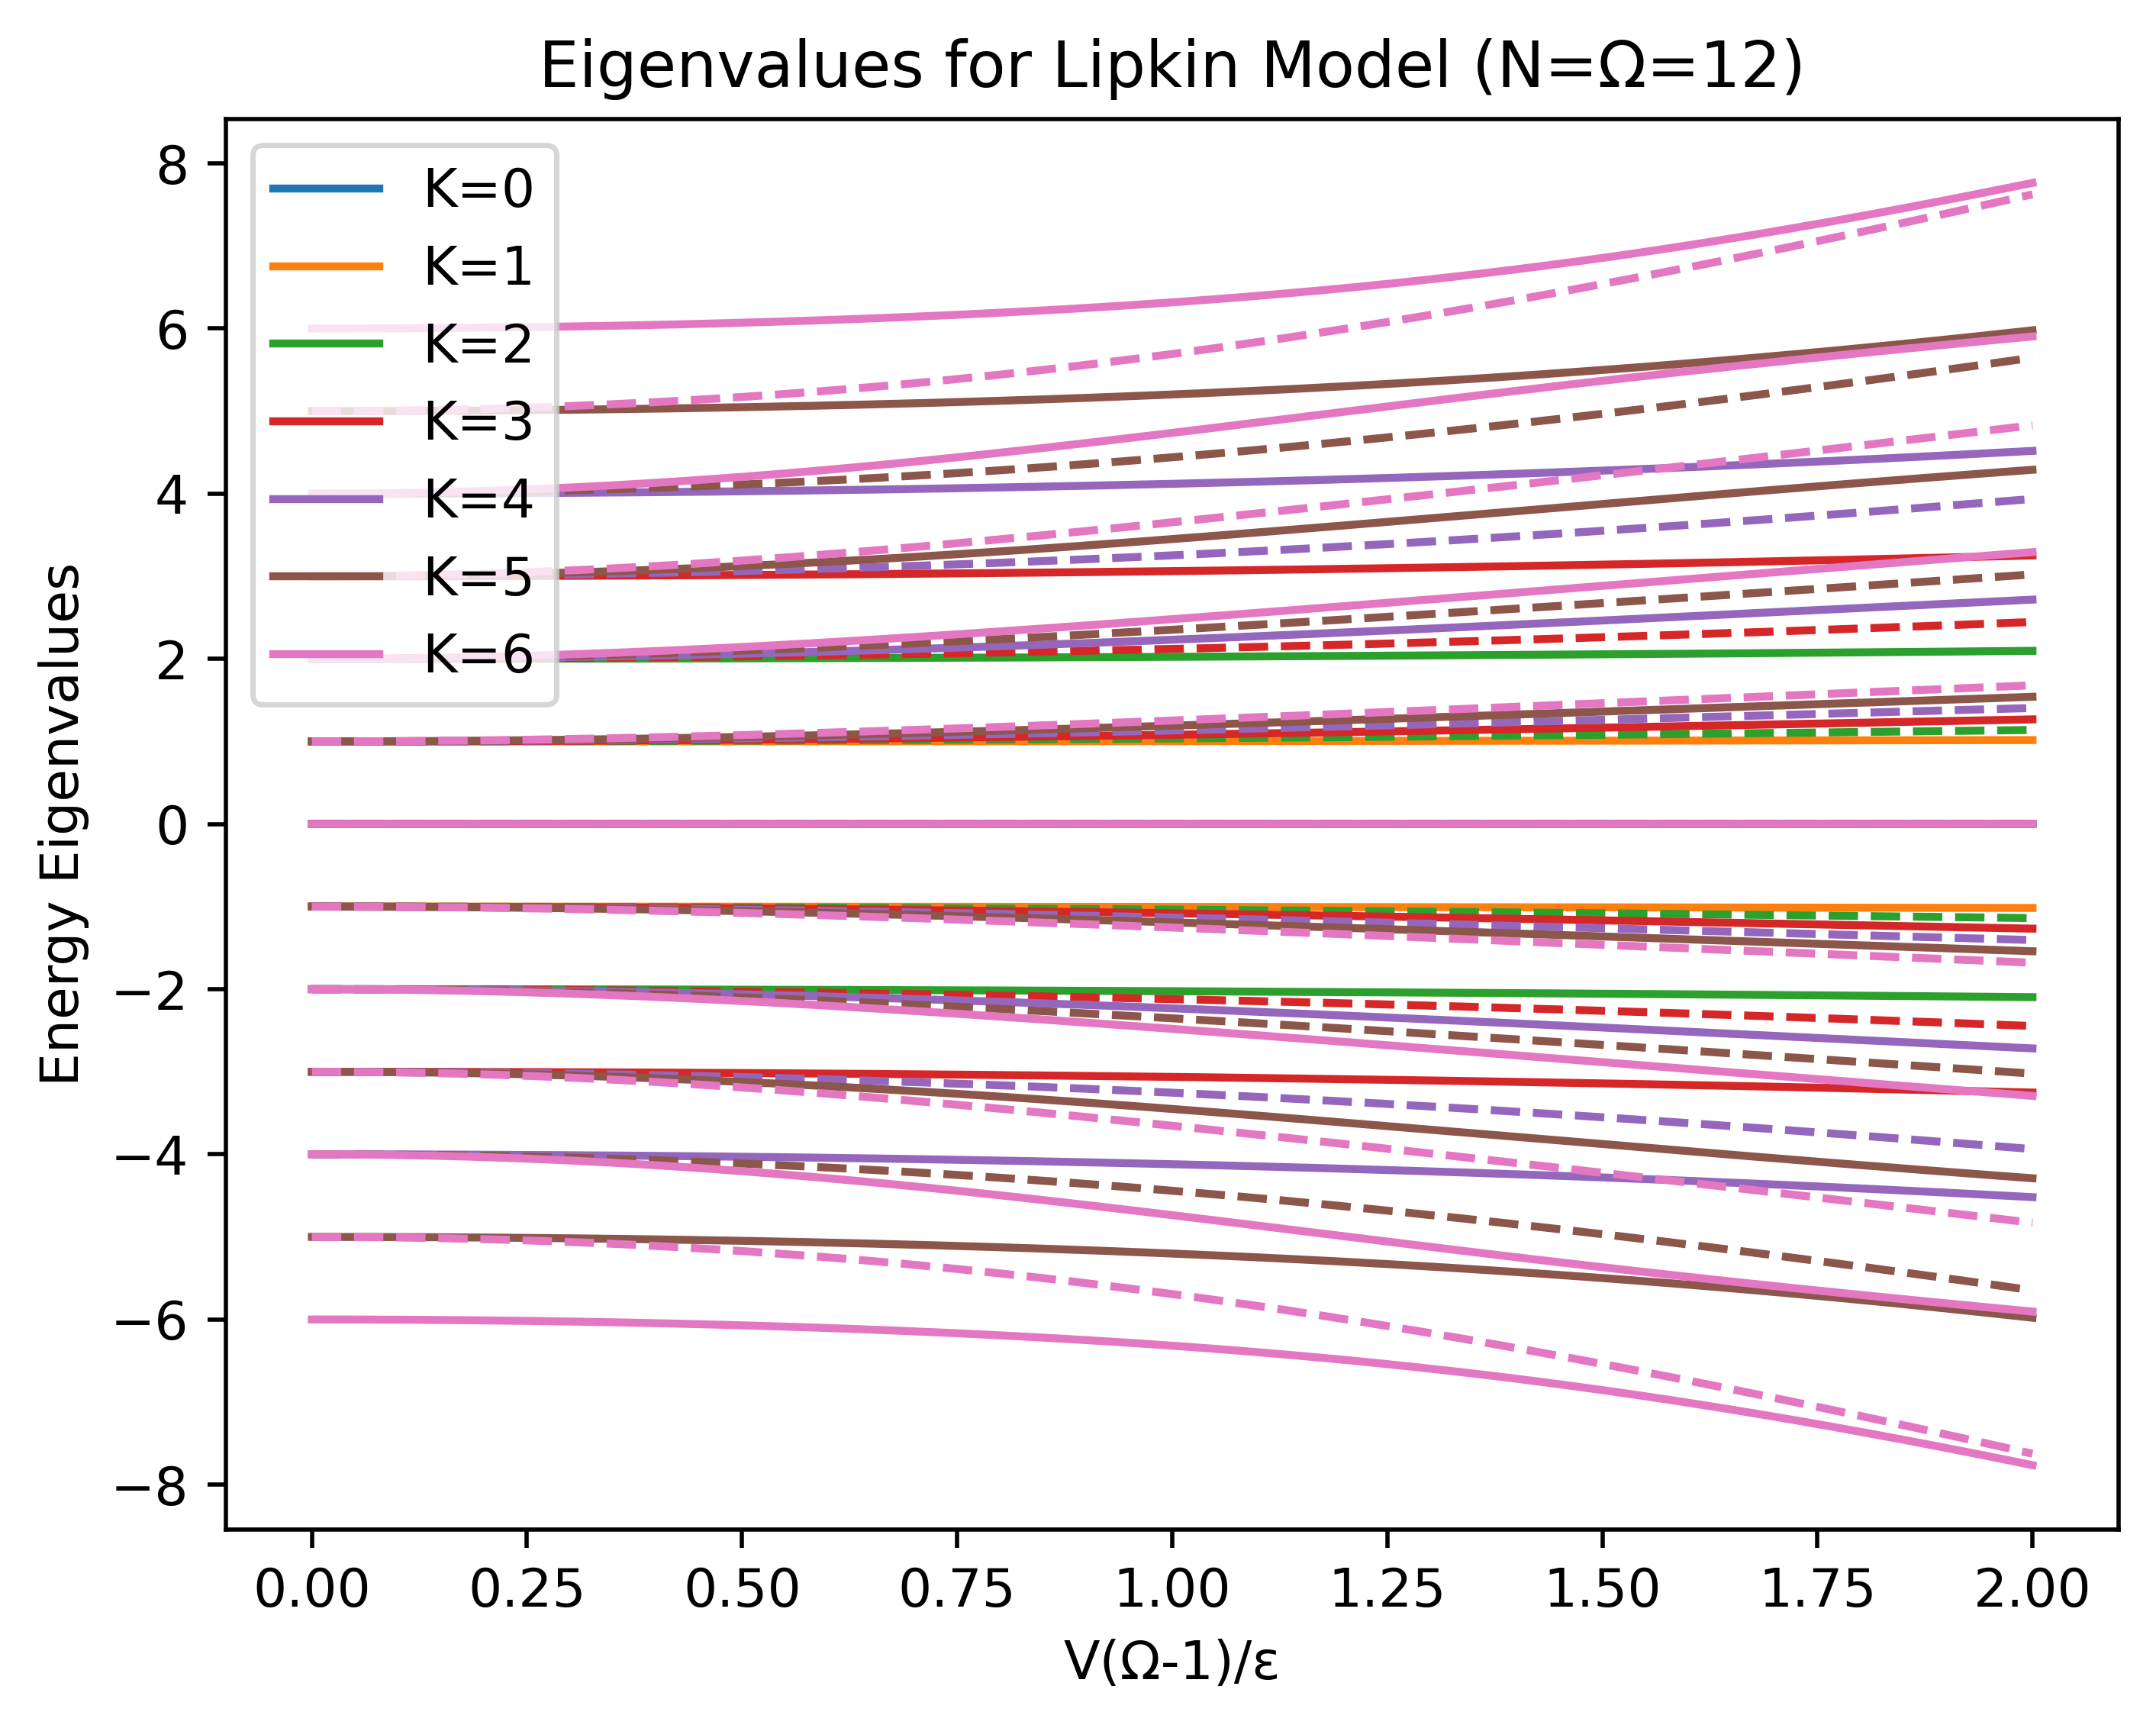
\includegraphics[width=0.8\linewidth]{figures/eigenvaluePlotAllK.png}
	\caption{
		In this figure, all values of $K$ are plotted in different colors, and dotted lines are $r=-1$.
	}
	\label{fig: eigenvalues all K}
\end{figure}

At a value of $V(\Omega-1)/\epsilon = 1$, the two smallest and two largest eigenvalues start becoming noticably closer together, and the difference between them continues to decrease as this $V$ increases, seemingly becoming arbitraily close.


\section{Transition Operator}\label{sec: transition}


The $\hat{K}_1$ operator is sometimes called the "transition" operator.
The reason for this is unknown to me.

For the ground state of the Hamiltonian, regardless of the number of particles, value of $\epsilon$, or value of $\Omega$, the expectation value of this operator is zero.
The argument for this comes from the angular momentum argument.
The ground state is when all particles have $\sigma = -1$, and this is an eigenstate of the $\hat{K}_3$.
Essentially, this state is anti-aligned with the $k_3$ axis, so measuring a positive value along the $k_1$ is just as likely as measuring a negative value.
Hence, the expectation value (with the ground state) for this operator is zero, always.

\begin{figure}[H]
	\centering
	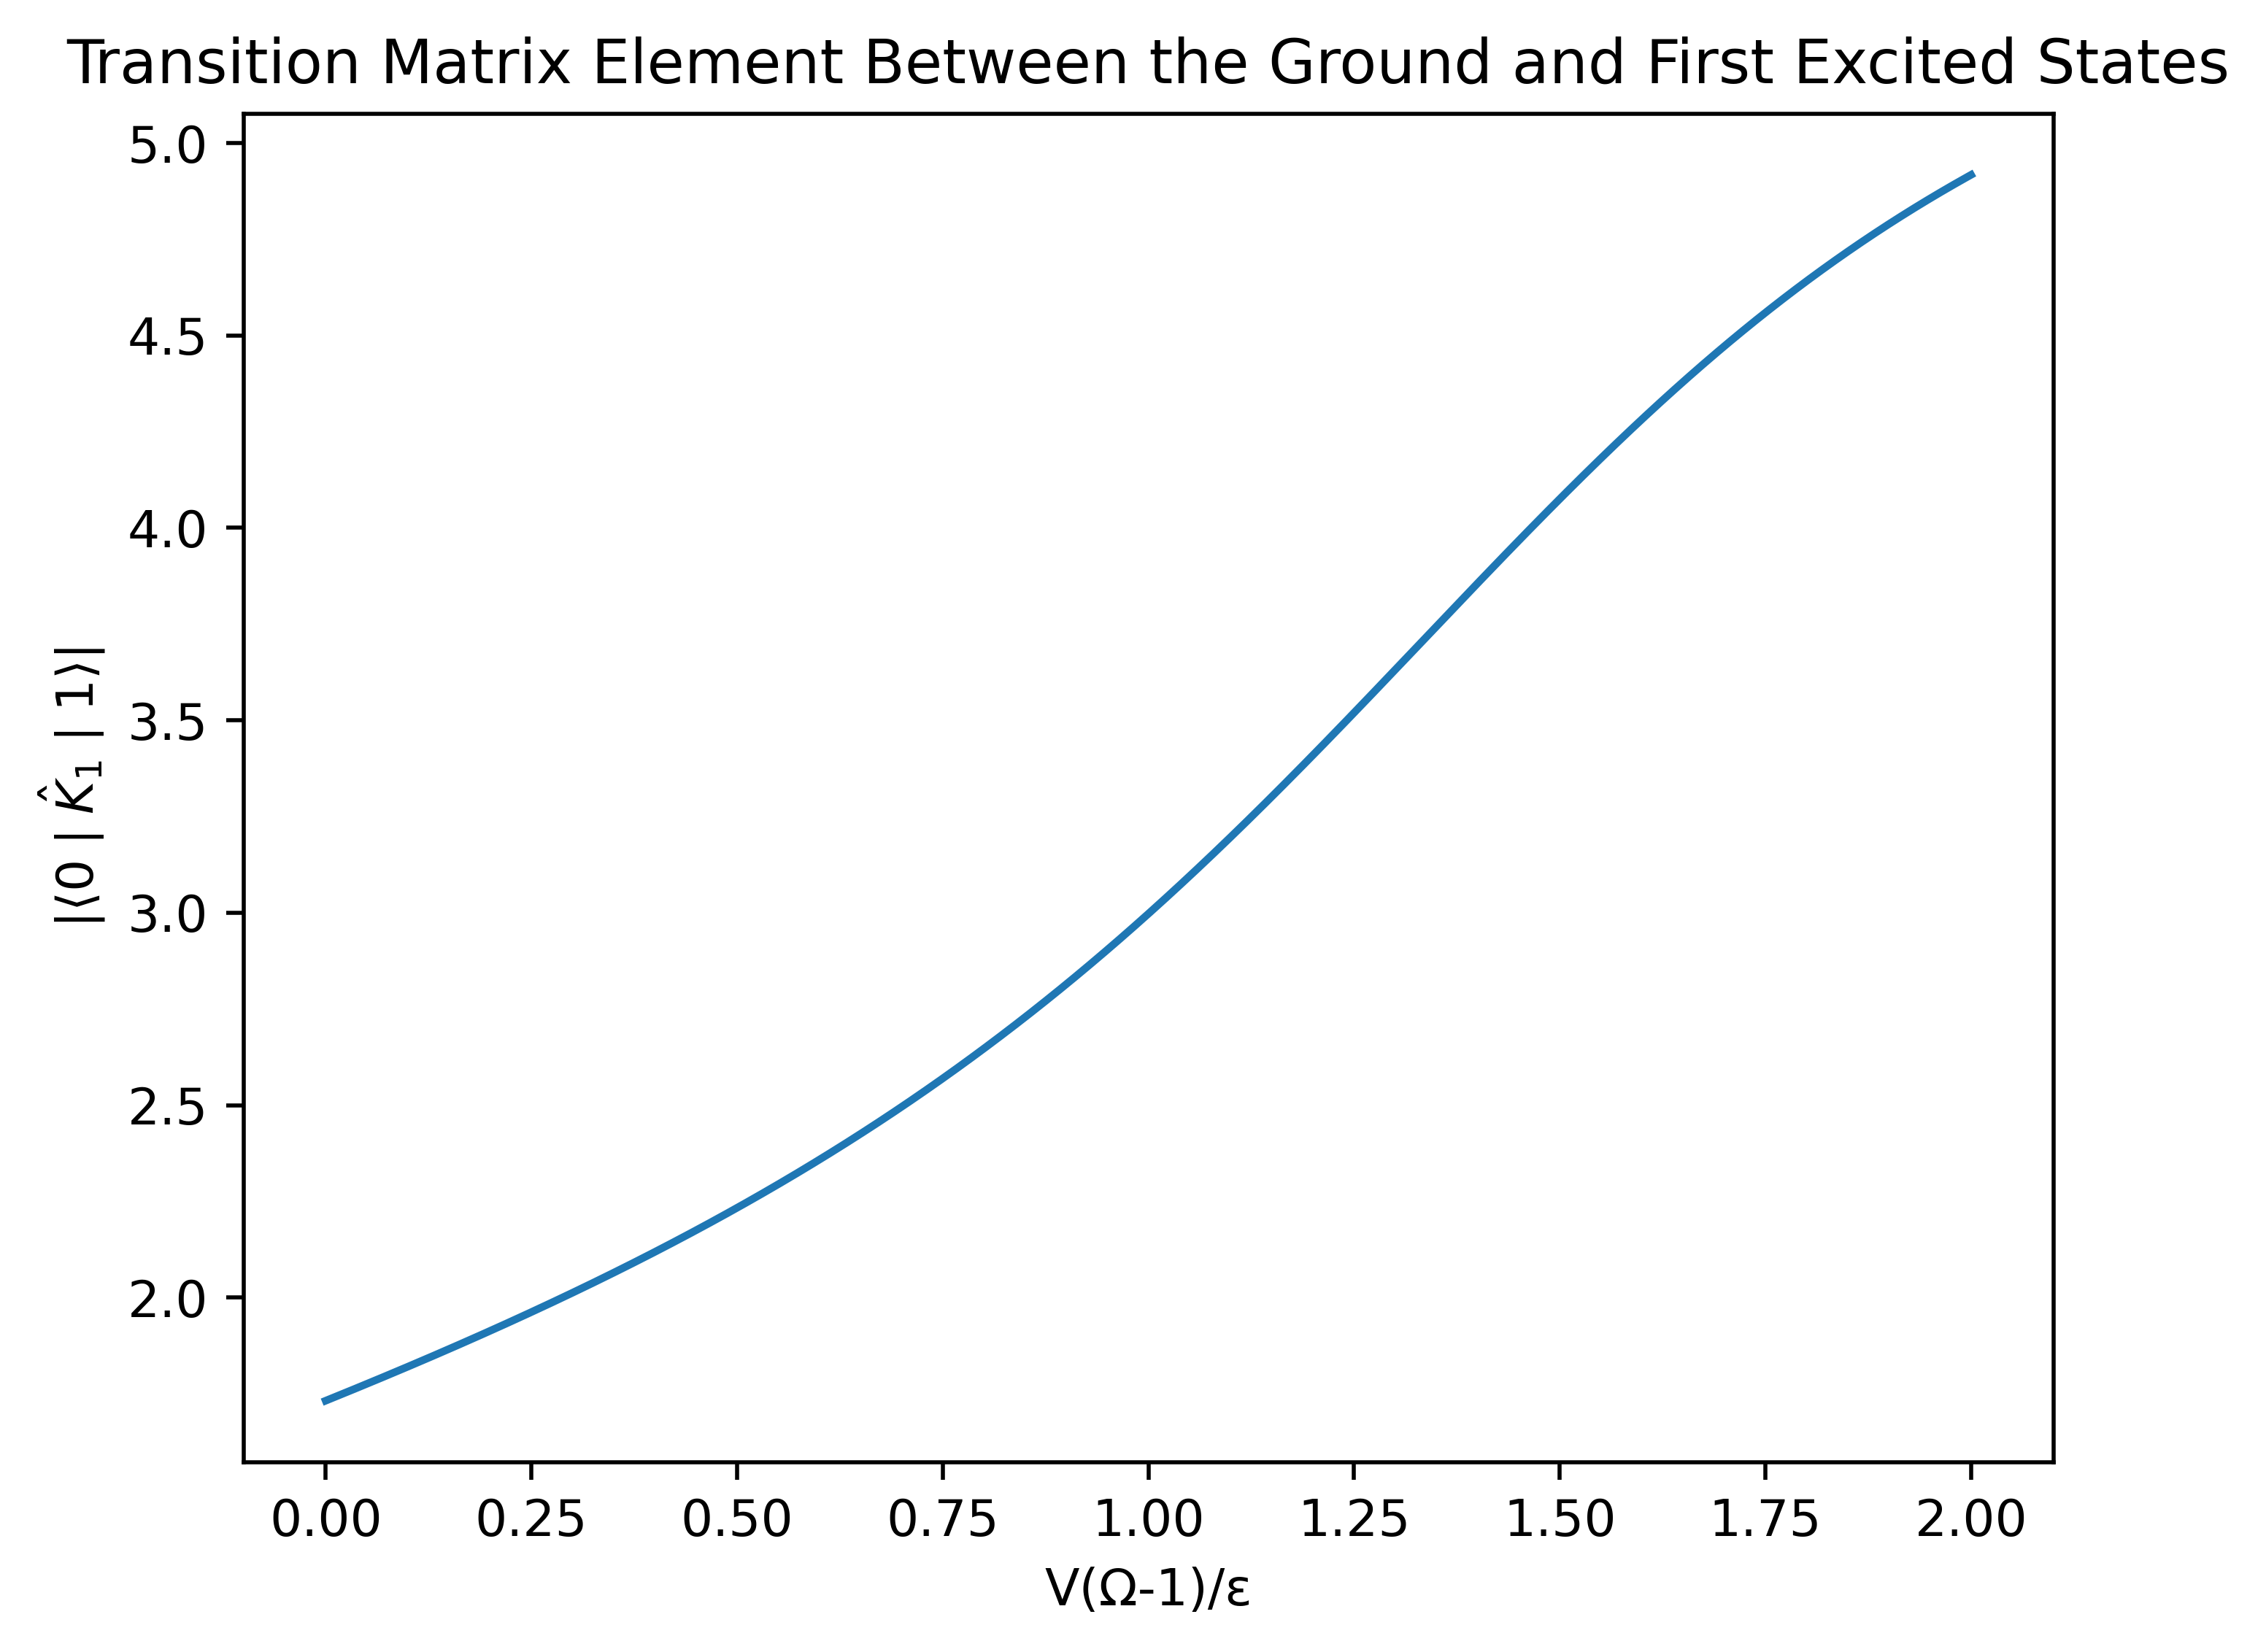
\includegraphics[width=0.8\linewidth]{figures/transitionMatrixElement.png}
	\caption{
		Here, the matrix element for the transition operator of the ground and first excited states is shown as a function of the $V(\Omega-1)/\epsilon$.
	}
	\label{fig: trans_mat_elem}
\end{figure}


\section{Comparison With the Occupation Basis}

In the occupation basis, one considers each possible state that the system can be in by considering how many ways one can place $N$ particles in $2\Omega$ states, accounting for the restricting one particle per state.

In the case of $N=\Omega=2$, there are six allowed states:
\begin{align*}
	\ket{1010}, \\
	\ket{1001}, \\
	\ket{0110}, \\
	\ket{0101}, \\
	\ket{1100}, \\
	\ket{0011}. 
\end{align*}
In the case of $N=4$ and $\Omega = 2$, there is only one allowed state:
\begin{align*}
	\ket{1111}.
\end{align*}

Consider the $N=4$ case, first.
In this system, all possible states are occupied, and there is no ability to move particles around.
Hence, the Hamiltonian in this basis is just the scalar $0$ (eigenvalue of zero (obviously)).

In the system where $N=2$, however, things are a little more interesting.
Being that there are more states, one can move between them by use of the $\hat{K}_\pm$ operators.
In this basis, the $\hat{K}$ matrices are given by
\begin{align*}
	\hat{K}_3 &= 
	\begin{pmatrix}
		-1 & 0 & 0 & 0 & 0 & 0 \\
		 0 & 0 & 0 & 0 & 0 & 0 \\
		 0 & 0 & 0 & 0 & 0 & 0 \\
		 0 & 0 & 0 & 1 & 0 & 0 \\
		 0 & 0 & 0 & 0 & 0 & 0 \\
		 0 & 0 & 0 & 0 & 0 & 0 \\
	\end{pmatrix}, \\
	\hat{K}_+ &= 
	\begin{pmatrix}
		 0 & 0 & 0 & 0 & 0 & 0 \\
		 1 & 0 & 0 & 0 & 0 & 0 \\
		 1 & 0 & 0 & 0 & 0 & 0 \\
		 0 & 1 & 1 & 0 & 0 & 0 \\
		 0 & 0 & 0 & 0 & 0 & 0 \\
		 0 & 0 & 0 & 0 & 0 & 0 \\
	\end{pmatrix}, \\
	\hat{K}_- &= 
	\begin{pmatrix}
		 0 & 1 & 1 & 0 & 0 & 0 \\
		 0 & 0 & 0 & 1 & 0 & 0 \\
		 0 & 0 & 0 & 1 & 0 & 0 \\
		 0 & 0 & 0 & 0 & 0 & 0 \\
		 0 & 0 & 0 & 0 & 0 & 0 \\
		 0 & 0 & 0 & 0 & 0 & 0 \\
	\end{pmatrix} .
\end{align*}
One now can use these to calculate the Hamiltonian and to find the energy eigenvalues of this Hamiltonian.
Doing this, the eigenvalues (found numerically) are
\begin{align}
	\lambda \in \{\sim -1.005,0,0,0,0,\sim 1.005\}.
\end{align}

Compare that with the method described in the rest of this paper.
There are three states with total $K = 1$, and one state with total $K = 0$.
The eigenvalues for the $K=1$ states are
\begin{align}
	\lambda \in \{\sim -1.005,0,\sim 1.005\},
\end{align}
and the eigenvalue for the $K=1$ state is $\lambda = 0$.
The states with eigenvalues of $\pm 1.005$ have quantum numbers $K = 1$ and $K_0 = \pm 1$, respectively.
The signature quantum number for both of these states is $r = 1$.

Notably, the occupation basis has two additional states that do not appear in the quasi-spin basis.
Those two states are $\ket{1100}$ and $\ket{0011}$: the states with two particles with the same value for $m$.
In these states, the total energy is zero, because there are the same number of particles with $\epsilon/2$ energy as there are with $-\epsilon/2$ energy, and there is no ability to move particles from $\sigma$ to $\sigma' \neq \sigma$.
One can argue that states in the $k$ basis which have an energy of zero are accounting for all states with such energy, i.e., ($\ket{KK_0}$)
\begin{align}
	\ket{10} &= \frac{1}{\sqrt{2}} (\ket{1001}+\ket{1100}),\\
	\ket{00} &= \frac{1}{\sqrt{2}} (\ket{0110}+\ket{0011}),
\end{align}
or something along these lines.


\section{Appendix}\label{sec: appendix}

\subsection{Commutation Relations} \label{ssec: appendix commutation}


\begin{align}
	[\hat{K}_+,\hat{K}_-]
		&= \sum_{m,n=1}^\Omega a_{m+}^\dagger a_{m-} a_{n-}^\dagger a_{n+} - a_{n-}^\dagger a_{n+} a_{m+}^\dagger a_{m-},\\
		&= \sum_{m,n=1}^\Omega a_{m+}^\dagger (\delta_{m-n-} - a_{n-}^\dagger a_{m-}) a_{n+}\nonumber\\
		&- \sum_{m,n=1}^\Omega a_{n-}^\dagger (\delta_{m+n+} - a_{m+}^\dagger a_{n+}) a_{m-},\\
		&= \sum_{m=1}^\Omega a_{m+}^\dagger a_{m+} - a_{m-}^\dagger a_{m-}\nonumber\\
		&+ \sum_{m,n=1}^\Omega a_{n-}^\dagger a_{m+}^\dagger a_{n+} a_{m-} - a_{m+}^\dagger a_{n-}^\dagger a_{m-} a_{n+},\\
		&= 2\hat{K}_3 + 0,\\
		&= 2\hat{K}_3.
\end{align}

\begin{align}
	[\hat{K}_3,\hat{K}_\pm]
		&= \frac{1}{2} \sum_{m,n=1}^\Omega (a_{m+}^\dagger a_{m+}-a_{m-}^\dagger a_{m-}) a_{n\pm}^\dagger a_{n\mp} \nonumber\\
		&- \frac{1}{2} \sum_{m,n=1}^\Omega a_{n\pm}^\dagger a_{n\mp} (a_{m+}^\dagger a_{m+}-a_{m-}^\dagger a_{m-}),\\
		&= \frac{1}{2} \sum_{m,n=1}^\Omega (a_{m+}^\dagger a_{m+} a_{n\pm}^\dagger a_{n\mp} - a_{m-}^\dagger a_{m-} a_{n\pm}^\dagger a_{n\mp}) \nonumber\\
		&- \frac{1}{2} \sum_{m,n=1}^\Omega (a_{n\pm}^\dagger a_{n\mp} a_{m+}^\dagger a_{m+} - a_{n\pm}^\dagger a_{n\mp} a_{m-}^\dagger a_{m-})\\
		&= \frac{1}{2} \sum_{m,n=1}^\Omega (a_{m+}^\dagger \delta_{m+n\pm} a_{n\mp} - a_{m-}^\dagger \delta_{m-n\pm} a_{n\mp} \nonumber\\
		&\qquad - a_{m+}^\dagger a_{n\pm}^\dagger a_{m+} a_{n\mp} + a_{m-}^\dagger a_{n\pm}^\dagger a_{m-} a_{n\mp}) \nonumber\\
		&- \frac{1}{2} \sum_{m,n=1}^\Omega (a_{n\pm}^\dagger \delta_{n\mp m+} a_{m+} - a_{n\pm}^\dagger \delta_{n\mp m-}a_{m-} \nonumber\\
		&\qquad - a_{n\pm}^\dagger a_{m+}^\dagger a_{n\mp} a_{m+} + a_{n\pm}^\dagger a_{m-}^\dagger a_{n\mp} a_{m-}),\\
		&= \pm \sum_{m=1}^\Omega a_{m\pm}^\dagger a_{\mp} \nonumber\\
		&+ \frac{1}{2} \sum_{m,n=1}^\Omega (a_{m-}^\dagger a_{n\pm}^\dagger a_{m-} a_{n\mp} - a_{m+}^\dagger a_{n\pm}^\dagger a_{m+} a_{n\mp}) \nonumber\\
		&+ \frac{1}{2} \sum_{m,n=1}^\Omega (a_{n\pm}^\dagger a_{m+}^\dagger a_{n\mp} a_{m+} - a_{n\pm}^\dagger a_{m-}^\dagger a_{n\mp} a_{m-}),\\
		&= \pm \hat{K}_\pm.
\end{align}

% \printbib
\stopmcols

\end{document}